\documentclass[12pt,a4paper]{book}
\usepackage[utf8]{inputenc}
\usepackage[spanish]{babel}
\usepackage{url}
\usepackage{times}
\usepackage{graphicx}
\usepackage{float}  %% H para posicionar figuras
\usepackage[nottoc, notlot, notlof, notindex]{tocbibind} %% Opciones de índice
\usepackage{latexsym}  %% Logo LaTeX
\usepackage[left=2cm,right=2cm,top=2cm,bottom=2cm]{geometry}

\title{Práctica 6.\\ Análisis Factorial}
\author{Sandra Gómez Gálvez & Sergio Casado López}

\renewcommand{\baselinestretch}{1.5}  %% Interlineado

\begin{document}

%%%%PORTADA:
\begin{titlepage}
\begin{center}
\begin{tabular}[c]{c c}


\includegraphics[scale=0.25]{urjc.png} 
\begin{tabular}[b]{l}
\Huge
\textsf{UNIVERSIDAD} \\
\Huge
\textsf{REY JUAN CARLOS} \\
\end{tabular}

\end{tabular}
\vspace{3cm}

\Large
INGENIERÍA DEL SOFTWARE Y MATEMÁTICAS

\vspace{0.4cm}

\large
Curso Académico 2018/2019

\vspace{0.8cm}



\vspace{2.5cm}

\LARGE
PRÁCTICA 6 - ANÁLISIS FACTORIAL

\vspace{4cm}

\large
Autores : Sandra Gómez Gálvez y Sergio Casado López\\
\end{center}
\end{titlepage}
\newpage
\mbox{}
\thispagestyle{empty} % para que no se numere esta pagina

%%%%%%%%%%%%%%%%%%%%%%%%%%%%%%%%%%%
%%%%%%%%%%%

\chapter{Análisis Factorial}
\label{sec:af} % etiqueta para poder referenciar luego en el texto con ~\ref{sec:r2}
\pagenumbering{arabic}
Realizaremos un análisis factorial a los datos para encontrar grupos de variables con un significado común y así reducir el número de dimensiones para explicar las respuestas de los sujetos. 
Para la realización de esta práctica utilizaremos el archivo\textit{ cereales2.txt} correspondientes a \textit{Datos práctica parcial}
\begin{figure}[H]
\centering
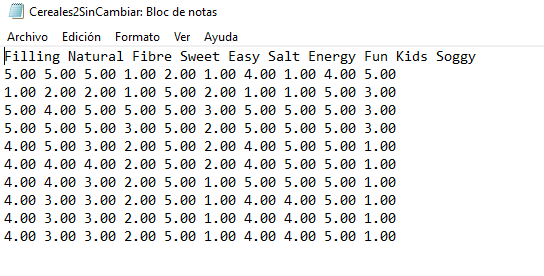
\includegraphics[scale=1]{Captura0.png} 
\caption{cereales2.txt}
\label{fig:c2txt}
\end{figure}
Para ello, en R, debemos importar la librería psych: 
\begin{figure}[H]
\centering

\includegraphics[scale=1]{Captura1.png} 
\caption{Libreria psych}
\label{fig:LibP}
\end{figure}
Cogeremos el fichero con los datos: 
\begin{figure}[H]
\centering
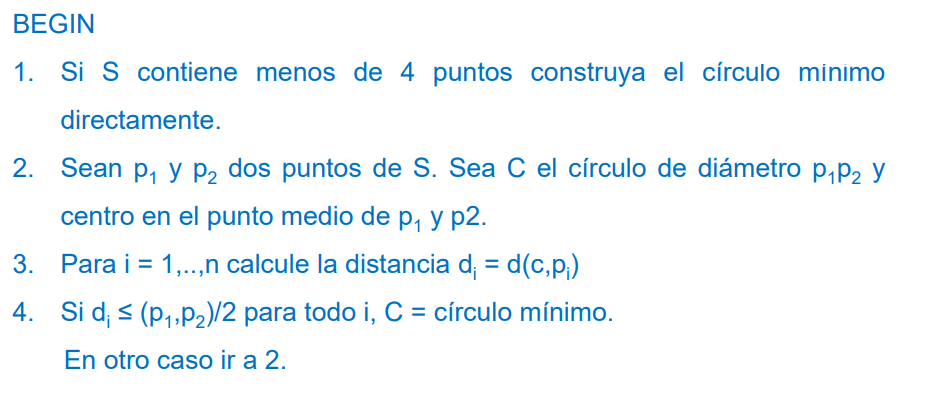
\includegraphics[scale=0.6]{Captura2.png} 
\caption{Fichero cereales2.txt}
\label{fig:c2}
\end{figure}
Sacamos su \textbf{determinante}: 
\begin{figure}[H]
\centering
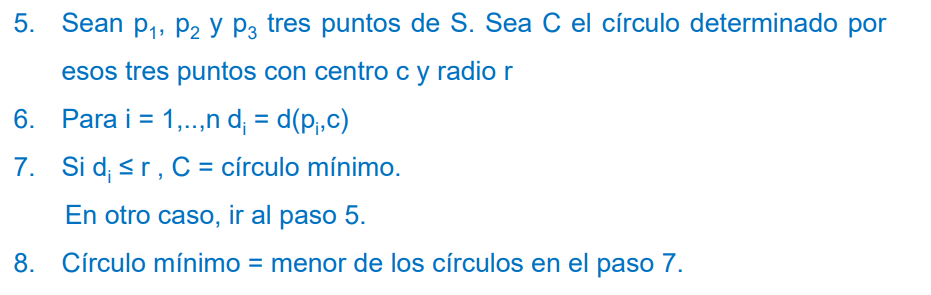
\includegraphics[scale=0.8]{Captura3.png} 
\caption{Determinante}
\label{fig:Det}
\end{figure}
Al hacer run al archivo en R, observamos como su determinante es 0.
\begin{figure}[H]
\centering
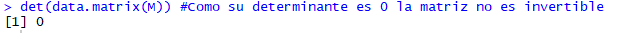
\includegraphics[scale=0.8]{Captura4.png} 
\caption{Determinante=0}
\label{fig:Det0}
\end{figure}
Esto implica que la matriz no será invertible, por ello, cambiaremos los datos en \textit{cereales2.txt} para que el determinante sea distinto de cero. Para ello, quitaremos las 2 últimas filas y las 2 últimas columnas ya que las 3 últimas filas son iguales entre ellas. 
\begin{figure}[H]
\centering
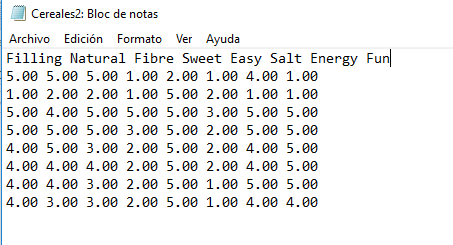
\includegraphics[scale=1]{Captura5.png} 
\caption{Nuevo cereales2.txt}
\label{fig:c2new}
\end{figure}
Por tanto, al hacer run al archivo R, nos sale determinante=216
\begin{figure}[H]
\centering
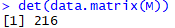
\includegraphics[scale=1]{Captura6.png} 
\caption{Determinante=216}
\label{fig:det216}
\end{figure}
Con el determinante ya distinto de 0, comenzaremos realizando el \textbf{Test de esfericidad de Bartlett}, con ello veremos si la matriz de correlación de las p variables observadas es la identidad. Contrastaremos si la matriz de correlación es la identidad
\begin{figure}[H]
\centering
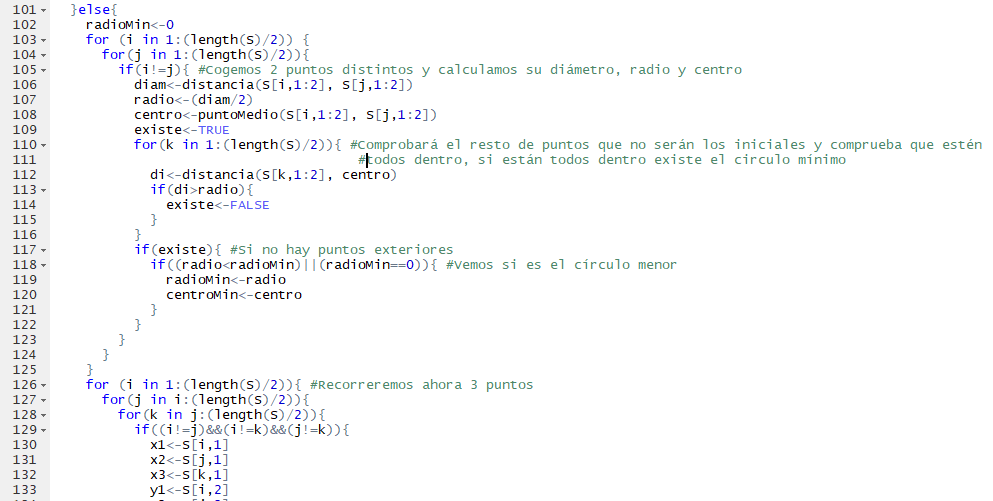
\includegraphics[scale=1]{Captura7.png} 
\caption{Test de esfericidad de Barlett}
\label{fig:bar}
\end{figure}
Que resulta en: 
\begin{figure}[H]
\centering
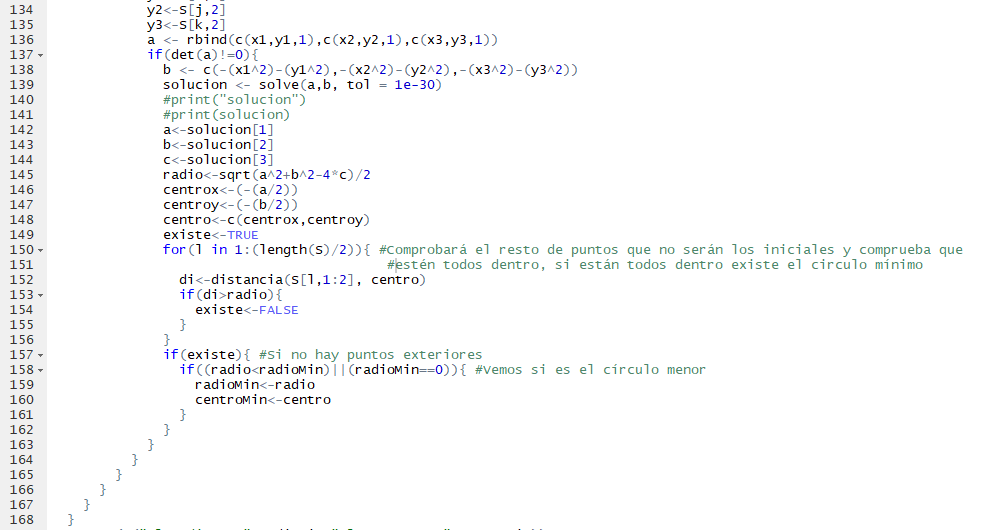
\includegraphics[scale=1]{Captura8.png} 
\caption{Resultados Test de esfericidad de Barlett}
\label{fig:barR}
\end{figure}
Desde la salida podemos ver que el valor de p de 0.5226 no es menor que el nivel de significación de 0.05. Esto significa que no podemos rechazar la hipótesis nula de que la varianza es la misma para todos los tipos de cereales.
\\Por tanto, podemos continuar con el análisis factorial. 
\textbf{Analizaremos los componentes principales sin rotar y los introduciremos en la variable} \textit{Modelo1}: 
\begin{figure}[H]
\centering
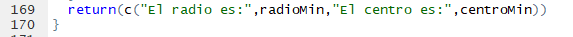
\includegraphics[scale=1]{Captura9.png} 
\caption{Ánalisis de componentes principales}
\label{fig:a1}
\end{figure}
Realizaremos la\textbf{ varianza }de cada componente: 
\begin{figure}[H]
\centering
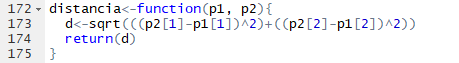
\includegraphics[scale=1]{Captura10.png} 
\caption{summary}
\label{fig:a1}
\end{figure}
Que resultará: 
\begin{figure}[H]
\centering
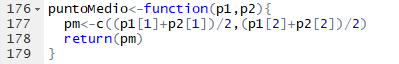
\includegraphics[scale=0.7]{Captura11.png} 
\caption{Varianza de cada componente}
\label{fig:v1}
\end{figure}
Observamos que estamos trabajando con 8 dimensiones, queremos saber si podemos trabajar con meno,  ¿con cuántas menos? 
\\Para ello, le \textbf{daremos puntuaciones a las componentes y crearemos un gráfico de sedimentación: }
\begin{figure}[H]
\centering
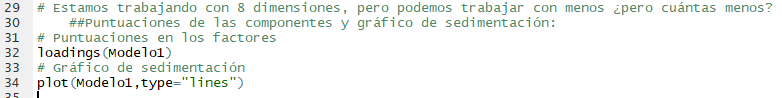
\includegraphics[scale=0.75]{Captura12.png} 
\caption{Puntuaciones y gráfico}
\label{fig:p1}
\end{figure}
Las puntuaciones y gráfico serán: 
\begin{figure}[H]
\centering
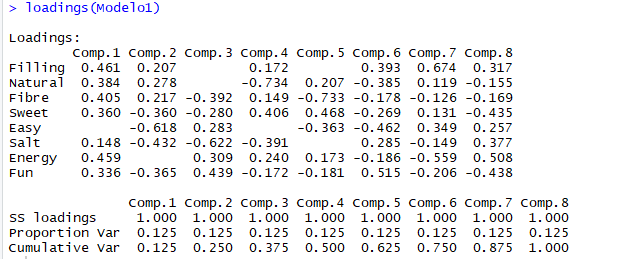
\includegraphics[scale=1]{Captura13.png} 
\caption{Puntuaciones}
\label{fig:p2}
\end{figure}
\begin{figure}[H]
\centering
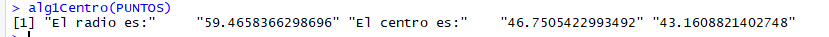
\includegraphics[scale=1]{Captura14.png} 
\caption{Gráfico}
\label{fig:g}
\end{figure}
\textbf{Estableceremos el número de factores en 2. 
Y utilizaremos una rotación \textit{varimax}}. Podríamos haber establecido la rotación como \textit{none, varimax,quartimax,promax,oblimin,simplimax, o cluster.} Pero elegimos \textit{varimax} porque así nos ajustaremos lo máximo posible a la realidad.
\\Por tanto, ahora, usando la libreria \textit{GPArotation} obtendremos un  \textit{Modelo2} con número de factores =2 y rotación varimax. 
\begin{figure}[H]
\centering
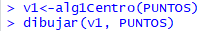
\includegraphics[scale=1]{Captura15.png} 
\caption{Factores=2 y Varimax}
\label{fig:vm}
\end{figure}
Que resultará en: 
\begin{figure}[H]
\centering
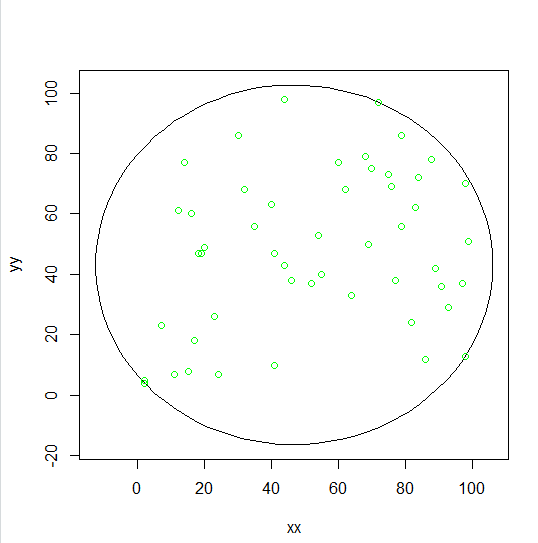
\includegraphics[scale=1]{Captura16.png} 
\caption{Modelo2}
\label{fig:mm}
\end{figure}
Además, podemos ver en que nos dice que la hipótesis de 2 factores es suficiente, por tanto es correcta.
\\Volvemos a realizar la \textbf{varianza de cada factor, las puntuaciones en los factores, las puntuaciones en cada caso, y un biplot para el \textit{Modelo2}:}
\begin{figure}[H]
\centering
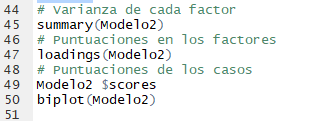
\includegraphics[scale=1]{Captura17.png} 
\caption{Varianza, puntuaciones factores, puntuaciones cada caso y Biplot}
\label{fig:vpp}
\end{figure}
Que resultan: 
\begin{figure}[H]
\centering
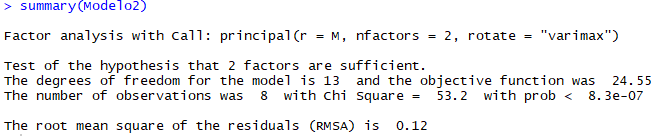
\includegraphics[scale=0.75]{Captura18.png} 
\caption{Resultado Varianza}
\label{fig:rv}
\end{figure}
\begin{figure}[H]
\centering
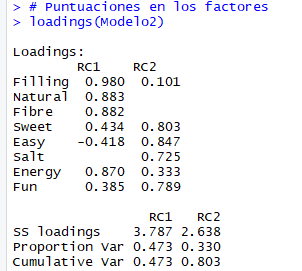
\includegraphics[scale=1]{Captura19.png} 
\caption{Puntuación en los factores}
\label{fig:pff}
\end{figure}
\begin{figure}[H]
\centering
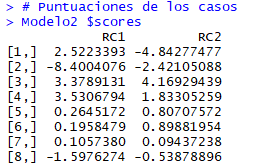
\includegraphics[scale=1]{Captura20.png} 
\caption{Puntuación de los casos}
\label{fig:pff}
\end{figure}
\begin{figure}[H]
\centering
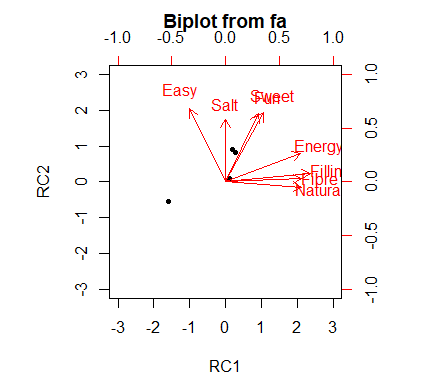
\includegraphics[scale=1]{Captura21.png} 
\caption{Biplot Modelo2}
\label{fig:pff}
\end{figure}
Por tanto, hemos podido reducir el Modelo a 2 casos funcionales. 
\\Ahora, queremos obtener el \textbf{análisis factorial basado en máxima verosimilitud. }
\\Para ello, realizaremos la función factanal con 4 factores y rotación varimax. No la podríamos realizar con más de 4 factores pues excedería. 
\begin{figure}[H]
\centering

\includegraphics[scale=0.75]{Captura22.png} 
\caption{Función factanal}
\label{fig:ff}
\end{figure}
Al hacer run sobre esta función encontraremos un error: 
\begin{figure}[H]
\centering
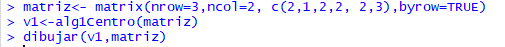
\includegraphics[scale=0.75]{Captura23.png} 
\caption{Error Función factanal}
\label{fig:errff}
\end{figure}
Esto indica que la matriz tiene que ser semidefinida positiva, para ello tendremos que cambiar/quitar algunas variables como hicimos anteriormente para que el determinante fuese distinto de 0. 
\\Tras varios intentos de cambios, esto no ha sido conseguido. En el caso de ser conseguido, los pasos siguientes serían: 
\begin{figure}[H]
\centering
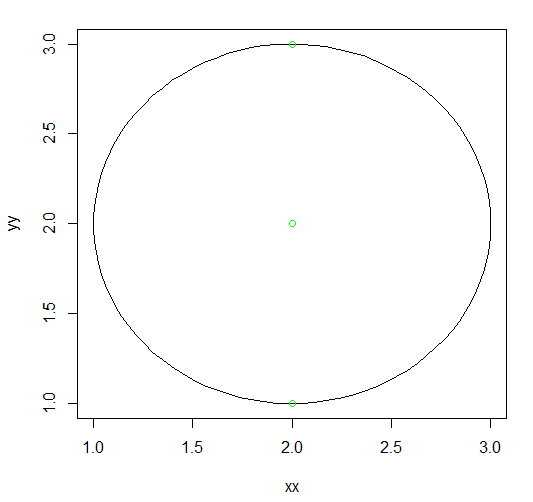
\includegraphics[scale=0.75]{Captura24.png} 
\caption{Pasos siguientes a la Función factanal}
\label{fig:psff}
\end{figure}
A pesar de no poder realizar el análisis factorial basado en máxima verosimilitud, hemos realizado un buen análisis factorial reduciendo todo a solamente 2 casos. 

\end{document}